%%%%%%%%%%%%%%%%%%%%%%%%%%%%%%%%%%%%%%%%%%%%%%%%%%%%%%%%%%%%%%%%%%%%%%
% LaTeX Example: Project Report
%
% Source: http://www.howtotex.com
%
% Feel free to distribute this example, but please keep the referral
% to howtotex.com
% Date: March 2011 
% 
%%%%%%%%%%%%%%%%%%%%%%%%%%%%%%%%%%%%%%%%%%%%%%%%%%%%%%%%%%%%%%%%%%%%%%
% How to use writeLaTeX: 
%
% You edit the source code here on the left, and the preview on the
% right shows you the result within a few seconds.
%
% Bookmark this page and share the URL with your co-authors. They can
% edit at the same time!
%
% You can upload figures, bibliographies, custom classes and
% styles using the files menu.
%
% If you're new to LaTeX, the wikibook is a great place to start:
% http://en.wikibooks.org/wiki/LaTeX
%
%%%%%%%%%%%%%%%%%%%%%%%%%%%%%%%%%%%%%%%%%%%%%%%%%%%%%%%%%%%%%%%%%%%%%%
% Edit the title below to update the display in My Documents
%\title{Project Report}
%
%%% Preamble
\documentclass[paper=a4, fontsize=11pt]{scrartcl}
\usepackage[T1]{fontenc}
\usepackage{fourier}
\usepackage{esdiff}
\usepackage[english]{babel}															% English language/hyphenation
\usepackage[protrusion=true,expansion=true]{microtype}	
\usepackage{amsmath,amsfonts,amsthm} % Math packages
\usepackage[pdftex]{graphicx}	
\usepackage{url}
\usepackage{caption}
\usepackage{float}



\usepackage{tikz}
\usepackage{pgfplots,pgfplotstable}
\usepackage{filecontents}

%%%%GFX

\usepackage[margin=0.5in]{geometry}
\usepackage[utf8]{inputenc}

\usepackage{pgfplots}
\pgfplotsset{width=10cm,compat=1.9}











%%% Custom sectioning
\usepackage{sectsty}
\allsectionsfont{\centering \normalfont\scshape}


%%% Custom headers/footers (fancyhdr package)
\usepackage{fancyhdr}
\pagestyle{fancyplain}
\fancyhead{}											% No page header
\fancyfoot[L]{}											% Empty 
\fancyfoot[C]{}											% Empty
\fancyfoot[R]{\thepage}									% Pagenumbering
\renewcommand{\headrulewidth}{0pt}			% Remove header underlines
\renewcommand{\footrulewidth}{0pt}				% Remove footer underlines
\setlength{\headheight}{13.6pt}


%%% Equation and float numbering
\numberwithin{equation}{section}		% Equationnumbering: section.eq#
\numberwithin{figure}{section}			% Figurenumbering: section.fig#
\numberwithin{table}{section}				% Tablenumbering: section.tab#


%%% Maketitle metadata
\newcommand{\horrule}[1]{\rule{\linewidth}{#1}} 	% Horizontal rule

\title{
		%\vspace{-1in} 	
		\usefont{OT1}{bch}{b}{n}
		\normalfont \normalsize \textsc{ECEN2350 Digital Logic Spring 2016} \\ [25pt]
		\horrule{0.5pt} \\[0.4cm]
		\huge Project 3 - The Reaction Timer \\
		\horrule{2pt} \\[0.5cm]
}
\author{
		\normalfont 								\normalsize
        Milan Formanek SID-103017710\\[-3pt]		\normalsize
        \today
}
\date{}


%%% Begin document
\begin{document}
\begin{center}
{\fontfamily{cmr}\selectfont}
\maketitle
\clearpage 
\section{Introduction}

The goal of this project is to create a reaction timer using the DE0 FPGA board. To make this work I will use more advanced features like the 50 mHz clock provided by the DE0 board as well as counters a binary to BCD decoder and a pseudo random number generator.

\section{Overview}

When the user releases the reset button, the device waits a random amount of time then flashes the LED and times the delay it takes the user to depress the "game" button. The delay between the the reset and the led bilking is to prevent the user from anticipating the exact time the reaction timer starts, thus truly testing his or her reaction time. After the users reaction time has been recorded the resultant reaction time is displayed in decimal form on the 7 segment screen.


\begin{figure}[h!]
\centering
\caption{Device diagram}
\includegraphics[scale=0.5]{diagram}
\label{fig:dia}
\end{figure}

\subsection{100 Hz Clock Divider}

The 50 mHz on board clock the DE0 provides, needs to be stepped down to a 100 Hz in order to trigger the Timer logic every $\frac{1}{100}$ of a second achieving the precision desired. This is implemented using a counter that overflows every 250000 cycles of the 50 mHz clock giving a final divided frequency of a 100 Hz.

\begin{figure}[h!]
\centering
\caption{50mHz to 100Hz divider verilog hardware description }
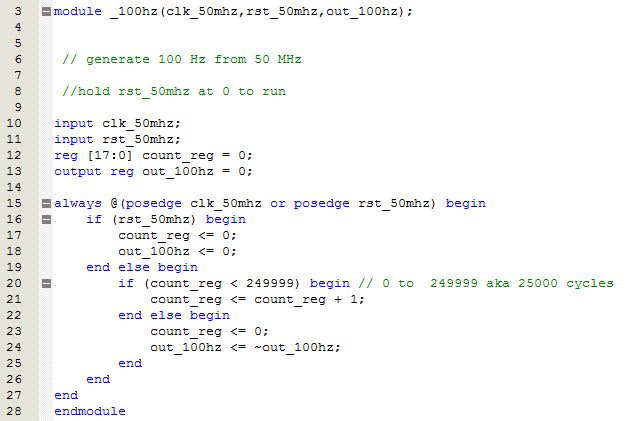
\includegraphics[scale=0.7]{divider}
\label{fig:div}
\end{figure}




\subsection{Pseudo Random Number Generator}

Using a linear feedback shift register (LFSR) you can generate a sequence of pseudo random numbers. This is achieved by shifting the data set in a shift register and XORing certain outputs with each other. I want to generate a 10 bit  random number, that will give me a max value of 1023 translating into the max go led delay of 10.23 sec. This is suitable to give enough of a range to provide enough randomness, but worst case scenario this still doesn't let the user wait too long. Using the Xilinx application notes or xapp052.pdf table 3 I find the right outputs to XOR. A LFSR can only be classified as a pseudo random number generator as it traverses $2^n-1$ states before repeating itself. Where n is the light of the shift register. I our case this would be $2^{10}-1$ states. Another thing to note is that if the shift register gets filled with only 0s the machine will lock up in that state forever. This is due to the fact that 0 XOR 0 = 0. 







\begin{figure}[h!]
\centering
\caption{Pseudo Random Number Generator Logic verilog hardware description}
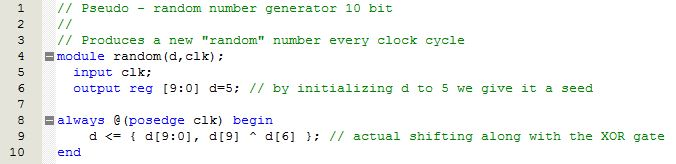
\includegraphics[scale=0.7]{ran}
\label{fig:ran}
\end{figure}


In Fig ~\ref{fig:unit}you can see the register is prevented from initializing in the lock up 0 state by setting the output register d to 5 initially. The shift register shifts down one every clock cycle producing a "fresh" random number.

To test if the LFSR worked I had a runtime that captured a random number every time I pressed the button and displayed it on the screen. Fig.~\ref{fig:histr} below presents a sample of random numbers generated by the LFSR. 

\pgfplotsset{compat=1.10}
\newcommand{\plots}{0.611201}
\newcommand{\plotm}{2.19882}
\begin{filecontents}{data.dat}
1 0.83
2 9.32
3 2.56
4 0.32
5 1.06
6 5.05
7 4.58
8 3.3
9 4.71
10 7.12

\end{filecontents}
\begin{figure}[h!]
\centering
\caption{Histogram of 10 sample random numbers from the generator}
\begin{tikzpicture}
\begin{axis}[
yticklabel style={/pgf/number format/fixed},
scaled y ticks = true,
minor y tick num={1},
xtick pos=left,
legend cell align = left,
legend style={draw=none},
xlabel = {},
ylabel = {},
ybar,
xtick={0,1,...,10},
ytick={0,1,...,10},
]
\addplot[blue,ybar,fill, fill opacity=0.3, bar width = 0.8] table {data.dat};

\legend{Random numbers}
\end{axis}
\end{tikzpicture}

\label{fig:histr}
\end{figure}









\subsection{Timer Logic}

The timer logic take care of the user input, flashing the go led, counting the time using the 100 Hz clock cycles and finally outputting the user reaction time in binary to the BCD decoder.  


\begin{figure}[h!]
\centering
\caption{State Diagram}
\includegraphics[scale=0.5]{states}
\label{fig:states}
\end{figure}

Fig ~\ref{fig:states} shows of the individual states of the reaction timer. The 10bit wide wire t represent the up to date "fresh" random number from the generator that is captured into the rdm register and led[9] represents the go led.


\begin{figure}[h!]
\centering
\caption{The Timer Logic verilog hardware description}
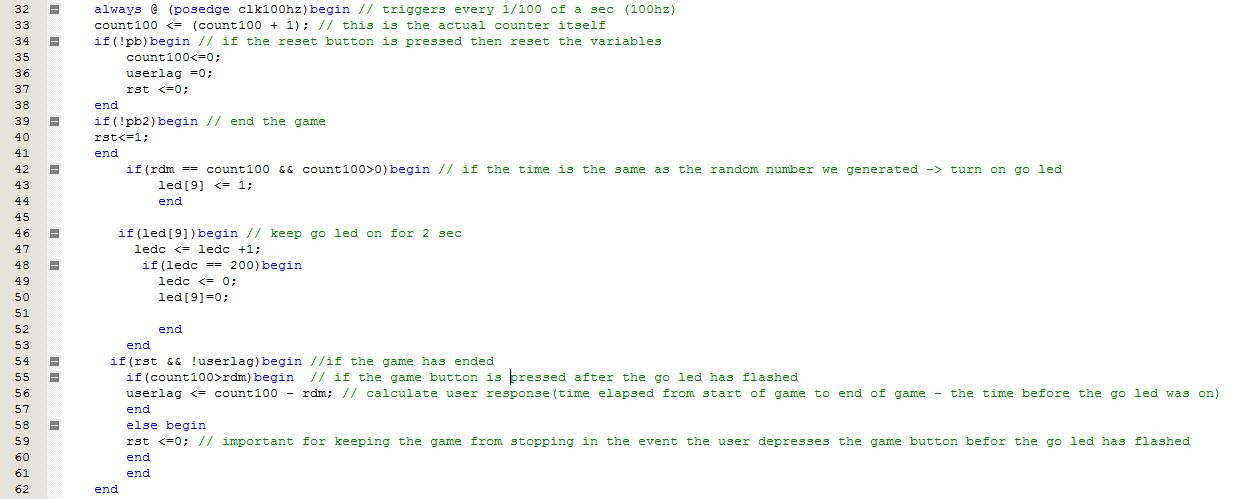
\includegraphics[scale=0.5]{code}
\label{fig:code}
\end{figure}

The number of clock cycles is stored in a 32 bit register. A number of this size will probably never get used and can't even be properly displayed on a 4 digit screen without overflow, nevertheless the counter will count up that high.



\subsection{Binary To Bcd Decoder}

The decoder gets a 14 bit number end converts it into 4 separate BCD digits. For this it uses the shift and add 3 method. The algorithm shifts the input and if the resultant shifted number is bigger than 4 it add 3 and then shift again. This process repeats itself until it has shifted the same amount of times as the input has binary digits.

\begin{figure}[h!]
\centering
\caption{shift and add 3 algorithm}
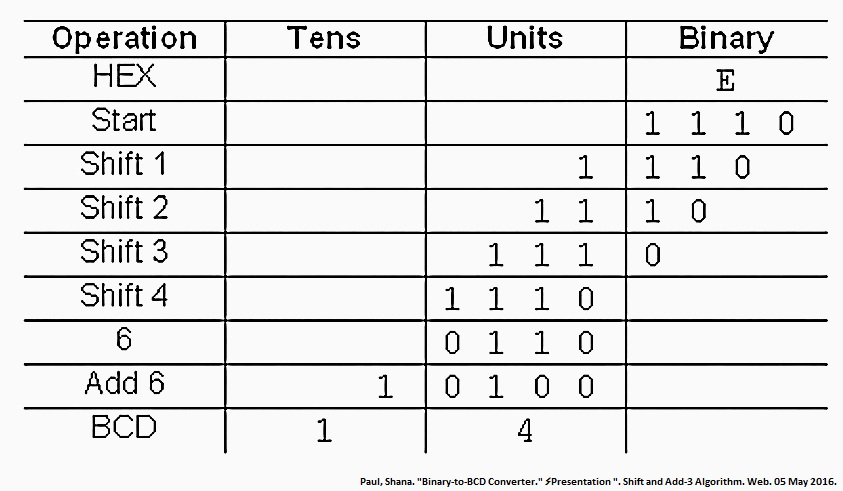
\includegraphics[scale=0.7]{add3}
\label{fig:add}
\end{figure}

Fig.~\ref{fig:add} above gives a visual representation of how the algorithm works converting $1110_2$ into BCD digits 1 and 4

\subsection{7 Segment decoder}

The decoder decodes input in the BCD (binary coded decimal) format to the 7 segment display. This is done using a bitmask on the led arrays that make up the screens themselves. The same logic was used in my project 1 and 2.



\section{User Manual}

After the device is turned on it waits for the user to press the reset button. Once the reset button is released (neg edge) the go led flashes after a random time interval. The device times how long it takes the user to depress (pos edge) the game button after the go led has turned on. The result is displayed on the 7 segment screen in seconds. Fig ~\ref{fig:unit} shows the physical layout of the device.

\begin{figure}[h!]
\centering
\caption{Overview}
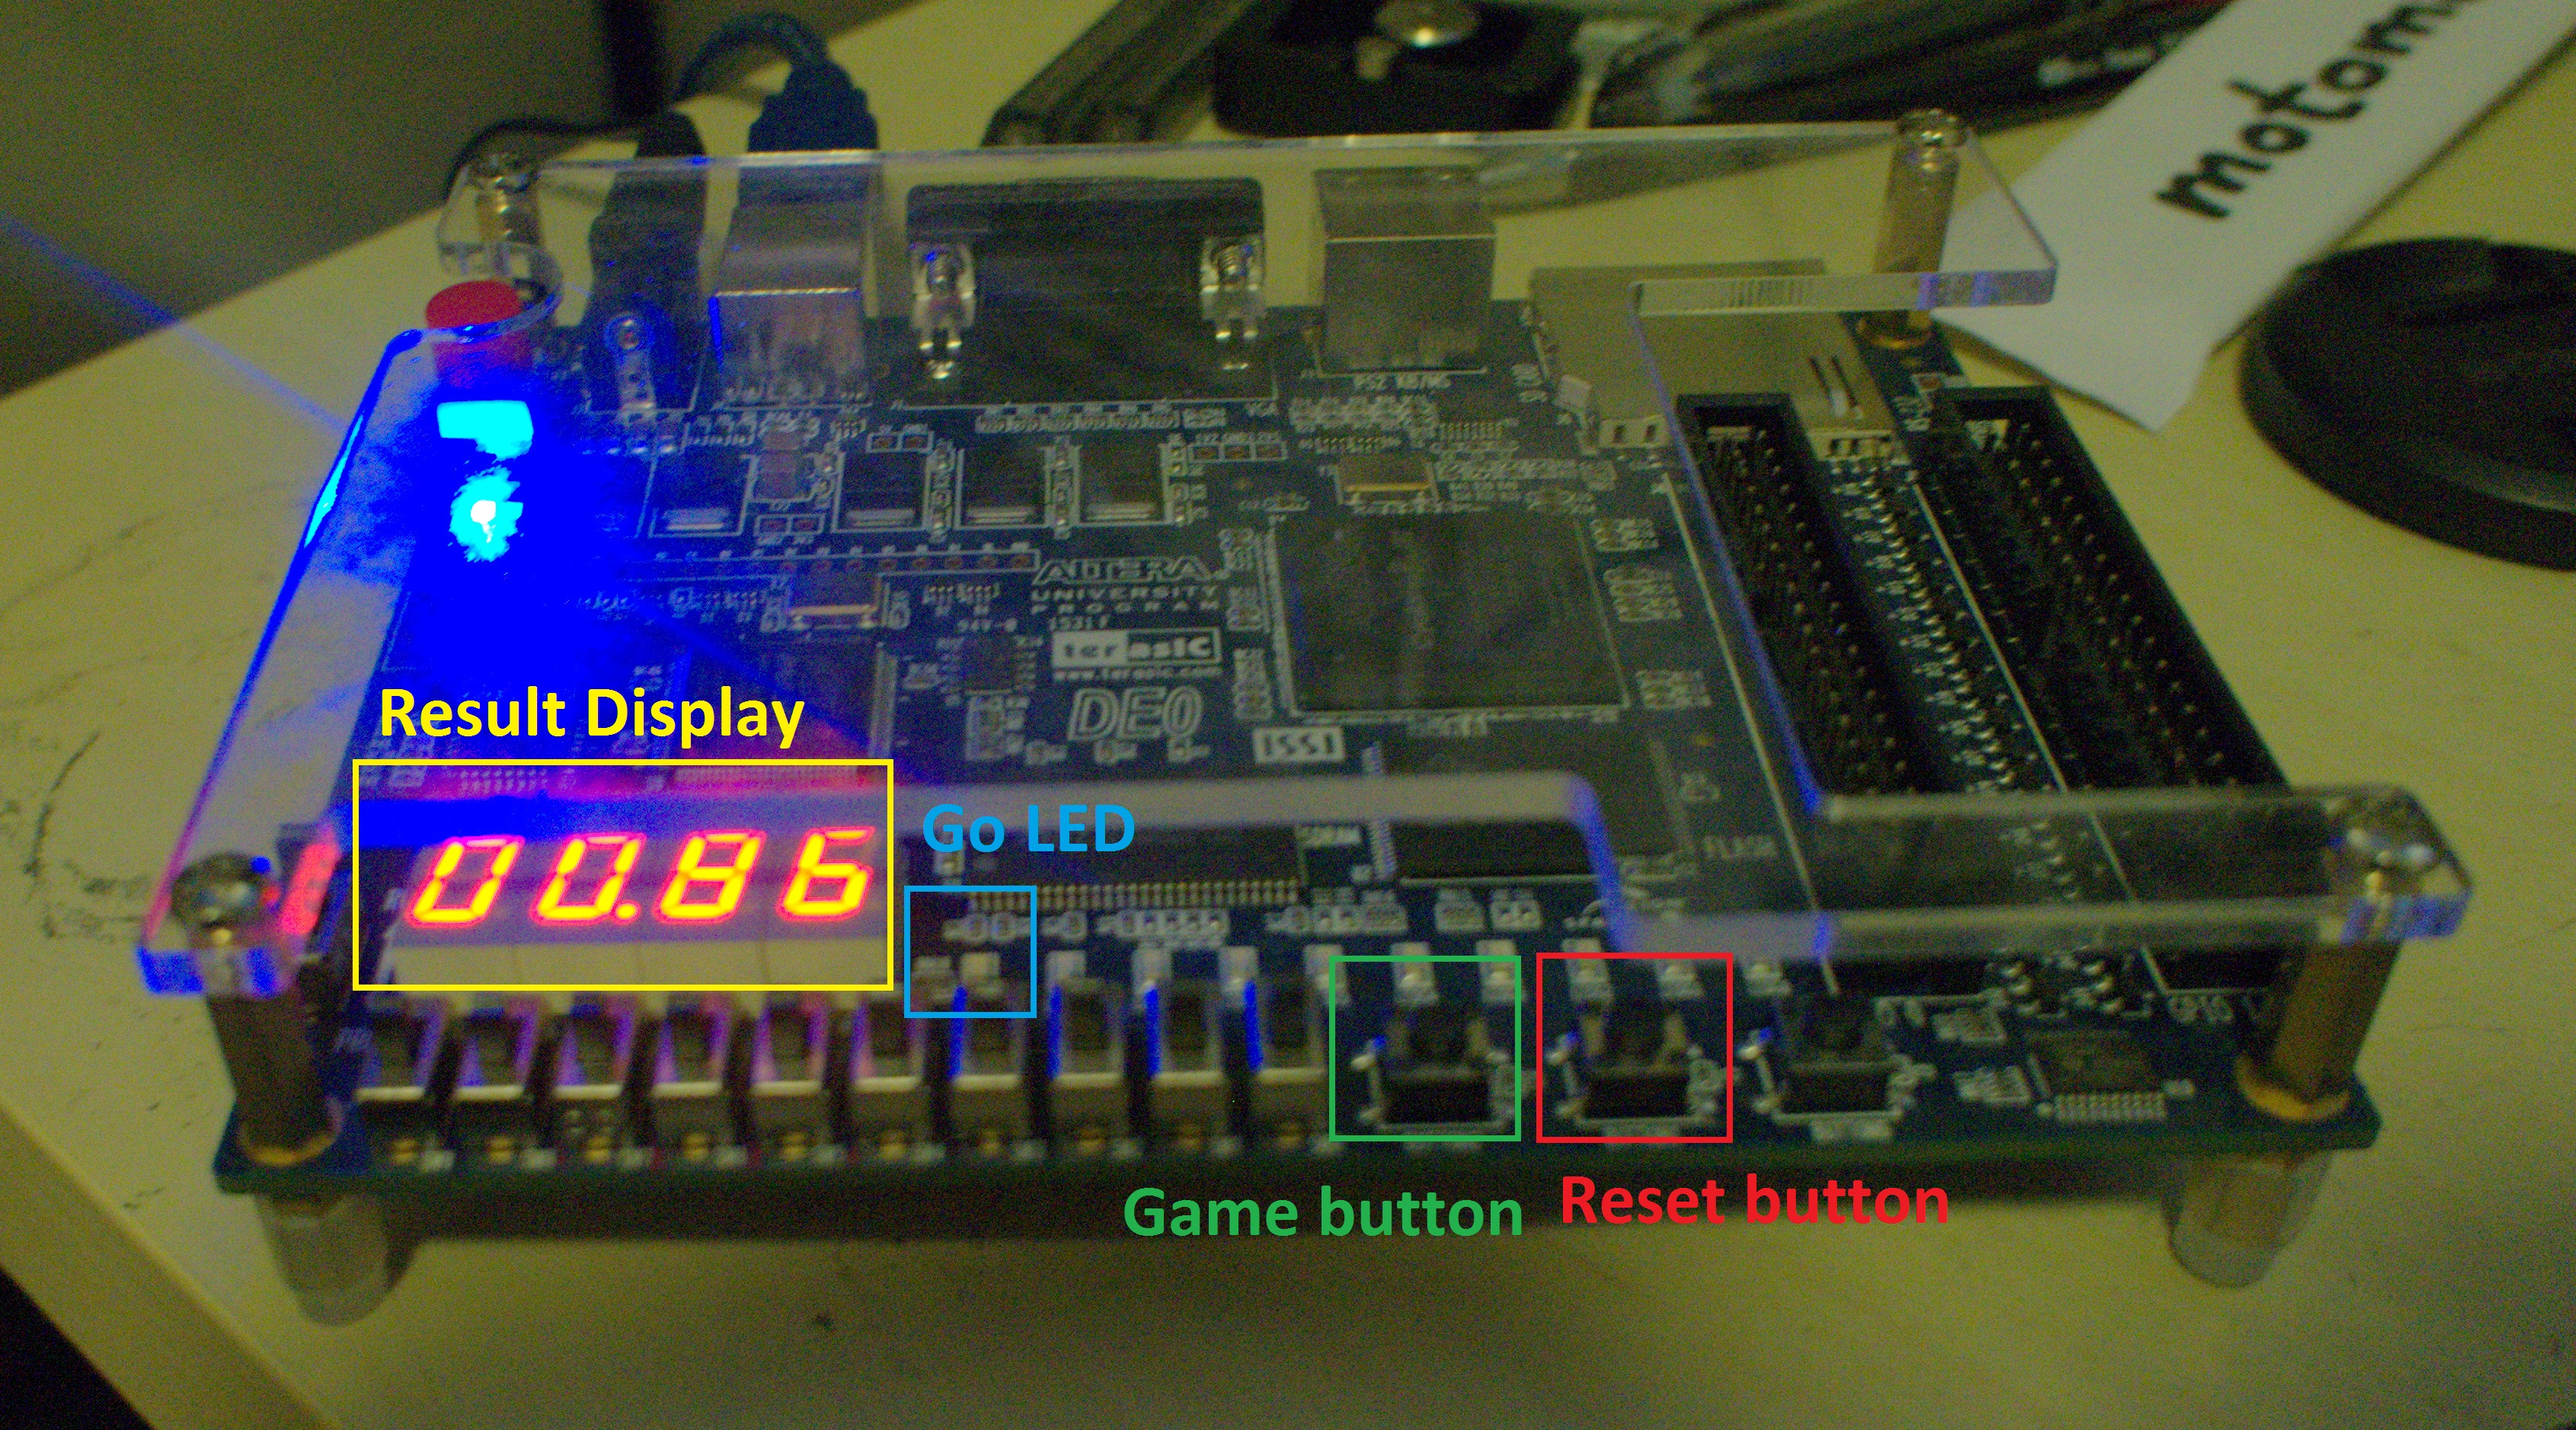
\includegraphics[scale=0.6]{unit}
\label{fig:unit}
\end{figure}


\section{Testing}

I have tested my reaction time at least 50 times. 10 of which are listed in fig.~\ref{fig:histm} below. I usually land somewhere between 0.23 sec and 0.28 sec. My best result is 0.21 sec and I finally had to give up on trying to break the 0.2 sec mark. I also tested with my flat mates and various friend with results varying from 0.20 sec to 0.53 sec. All the test subjects were in there 20s, it would be interesting to test with someone older to see if response time really decays with age. 

\pgfplotsset{compat=1.10}
\newcommand{\plots}{0.611201}
\newcommand{\plotm}{2.19882}
\begin{filecontents}{data.dat}
1 0.28
2 0.26
3 0.31
4 0.21
5 0.25
6 0.23
7 0.26
8 0.25
9 0.22
10 0.23

\end{filecontents}
\begin{figure}[h!]
\centering
\caption{10 of my response times}
\begin{tikzpicture}
\begin{axis}[
yticklabel style={/pgf/number format/fixed},
scaled y ticks = true,
minor y tick num={1},
xtick pos=left,
legend cell align = left,
legend style={draw=none},
xlabel = {},
ylabel = {},
ybar,
xtick={0,1,...,10},
ytick={0,0.02,...,1},
]
\addplot[blue,ybar,fill, fill opacity=0.3, bar width = 0.8] table {data.dat};

\legend{responce time in seconds}
\end{axis}
\end{tikzpicture}

\label{fig:histm}
\end{figure}




\section{Final remarks and conclusion}

After project 2 I had all but given up on my DE0 board. The switches did not work and the 7 segment screen flickered intermittently. I tested it with different code and determined it was a hardware issue and I just got a lemon. Before throwing in the towel and buying a new board I though I would try one last thing. After stripping the board down I put it in the oven for 8 minutes at 380 F to try re-flow the solder. I would say this is crazy but it worked. After letting the board cool down and reassembling it worked like new. As far as the project itself goes I found this one easier than project 2. Everything was straight forward, event the random number generator which I thought would be a challenge didn't take to long. Last semester I took the digital clock project class where I used a physical 7400 series counter chip to step down a 32 kHz clock from a RTC crystal and all I have to say is the process of making an equivalent circuit in verilog "software" is so much simpler and less hassle. I'm glad that I can finally present you with a project that is up to my standards.

%%% End document
\end{center}
\end{document}